%-----------------------------------------------------------------------------

\SVN $Id$
\rfoot{\SVNId}

\begin{ighsec}{Introduction}
\label{sec:intro}

The name EtherLab\regTM\ once stood for an open-source solution of using the
EtherCAT\regTM\ fieldbus technology with MATLAB/Simulink\regTM\ for automation
and test purposes. Today, EtherLab is much more than this: It is neither
depending on EtherCAT, nor on MATLAB/Simulink any more. Below is a short
summary of what EtherLab is capable of:

\begin{itemize}

\item Realtime execution of multiple models with multiple tasks inside the
Linux kernel.

\item Accessing the models' signals and parameters via TCP/IP. There is a
generic C++ library called RTCom and many tools for visualisation, data
logging, etc. available from \url{http://etherlab.org/en/components.php}.

\item Creation of realtime models with a C-API (see section~\ref{sec:api}).

\item Creation of realtime models using MATLAB/Simulink and the EtherLab
blockset (see section~\ref{sec:simulink}).

\end{itemize}

\end{ighsec}

%-----------------------------------------------------------------------------

\begin{ighsec}{Architecture}
\label{sec:arch}

The EtherLab package can be subdivided into the components listed below:

\begin{itemize}

\item The Linux kernel module \texttt{rt\_kernel}, that is responsible for the
realtime execution of the created models.

\item The EtherLab ``Buddy Process'', that acts as a userspace counterpart to
the \texttt{rt\_kernel} and is responsible for providing process data via
TCP/IP (see figure~\ref{fig:architektur}).

\item The EtherLab C-API, that is used to create realtime models, basically
consisting of tasks, signals and parameters. Models are described using and
EtherLab model XML file that is used to create the realtime data structures
and the model information for the buddy process.

\item The MATLAB/Simulink integration of EtherLab in terms of the
\texttt{etherlab\_lib} for Simulink (containing all necessary blocks) and the
EtherLab target for the Realtime Workshop, that is able to create EtherLab
models that will use the EtherLab C-API.

\end{itemize}

\begin{figure}[H]
  \begin{center}
    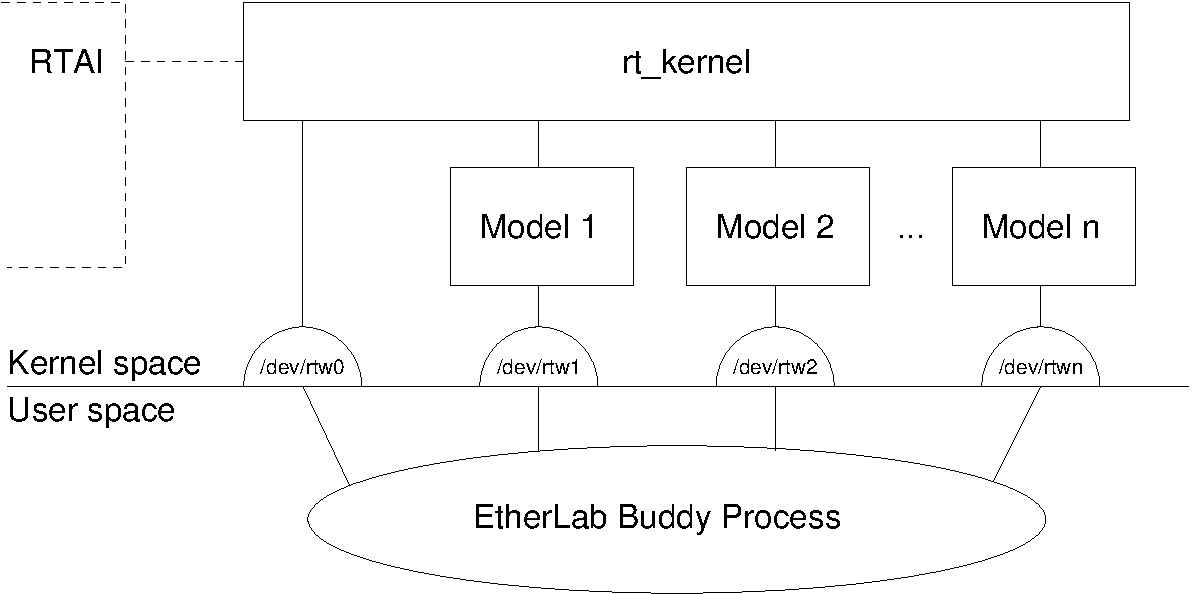
\includegraphics[width=\textwidth]{images/etl-arch}
    \caption{EtherLab runtime architecture}
    \label{fig:architektur}
  \end{center}
\end{figure}

\end{ighsec}

%-----------------------------------------------------------------------------

\begin{ighsec}{Installation}
\label{sec:install}

\begin{ighsec}{Prerequisites}

Prerequisites for the installation of EtherLab:

\begin{itemize}

\item Linux kernel 2.6 (including kernel sources)

\item RTAI $\ge$ 3.3

\item {\it optional:} MATLAB/Simulink with Realtime Workshop, if Simulink
shall be used to create EtherLab models. Recommended are MATLAB versions
2006{\it x} -- 2007{\it x}.

\item {\it optional:} EtherCAT master 1.4, if the Simulink EtherCAT blocks
shall be used. See \url{http://etherlab.org/en/ethercat}.

\end{itemize}

It is recommended to install EtherLab components to \texttt{/opt/etherlab}. If
this directory does not exist, it can be created with the commands below:

\begin{lstlisting}
  # `\textbf{mkdir /opt/etherlab}`
  # `\textbf{chown root:users /opt/etherlab}`
  # `\textbf{chmod 775 /opt/etherlab}`
\end{lstlisting}

\end{ighsec}

\begin{ighsec}{Installation}
\label{sec:inst-paket}

Installation is done after copying the EtherLab tarball from the EtherLab CD
(or downloading from \url{http://etherlab.org}) as normal user according to
the commands below. The last command installs EtherLab into the directory
\texttt{/opt/etherlab}. A different target directory can be selected via the
\texttt{--prefix} parameter of the \texttt{configure} script (see
\texttt{configure --help}).

\begin{lstlisting}
  `\$` `\textbf{tar xzf etherlab-\version.tar.gz}`
  `\$` `\textbf{cd etherlab-\version/}`
  `\$` `\textbf{./configure}`
  `\$` `\textbf{make}`
  `\$` `\textbf{make install}`
\end{lstlisting}

\end{ighsec}

\begin{ighsec}{Installation of the Simulink Library}
\label{sec:inst-blockset}

As a prerequisite for the \texttt{setup\_etherlab} command (see below) to
succeed, the file \texttt{toolbox/local/pathdef.m} inside the MATLAB
installation directory must be writable for the user running MATLAB. Enter the
below commands (as \textit{root}) to make it writable for all users in the
group \textit{users} (substitute the variable \texttt{\$MATLABDIR} with the
correct path first):

\begin{lstlisting}
  # `\textbf{chown :users \$MATLABDIR/toolbox/local/pathdef.m}`
  # `\textbf{chmod 664 \$MATLABDIR/toolbox/local/pathdef.m}`
\end{lstlisting}

To setup the EtherLab Simulink library \texttt{etherlab\_lib} for the use in
MATLAB, the below commands must be entered (out of MATLAB).

\begin{lstlisting}
  >> `\textbf{cd /opt/etherlab/rtw}`
  >> `\textbf{setup\_etherlab}`
\end{lstlisting}

\end{ighsec}

\begin{ighsec}{Starting EtherLab as a Service}
\label{sec:dienst}

If the EtherLab kernel/buddy are to be started as a service, the provided init
script \texttt{etherlab} can be used. However, the insertion of the service is
dependent on the GNU/Linux distribution used. The command sequence below is
intended for openSUSE Linux:

\begin{lstlisting}
  # `\textbf{ln -s /opt/etherlab/etc/init.d/etherlab /etc/init.d/}`
  # `\textbf{insserv etherlab}`
\end{lstlisting}

\end{ighsec}

\end{ighsec}

%-----------------------------------------------------------------------------

\begin{ighsec}{The EtherLab C-API}
\label{sec:api}

\ldots

\end{ighsec}

%-----------------------------------------------------------------------------

\begin{ighsec}{Simulink Integration}
\label{sec:simulink}

%-----------------------------------------------------------------------------

\begin{ighsec}{The Simulink Library}
\label{sec:lib}

The EtherLab library \texttt{etherlab\_lib} was designed to allow the creation
of EtherLab models using MATLAB/Simulink. For example, it contains blocks for
all supported EtherCAT slaves. To show the library window (see
figure~\ref{fig:blockset}), the command below have to be entered in
MATLAB:

\begin{lstlisting}
  >> `\textbf{etherlab\_lib}`
\end{lstlisting}

Figure~\ref{fig:blockset} shows the window containing the
\texttt{etherlab\_lib} with the EtherCAT blockset. Each block has a
configuration dialog, that shows up after double-clicking on the block area.
There is a ``Help'' button in all of the configuration dialogs, that provides
detailed help concerning the dialog elements.

\begin{figure}[H]
  \begin{center}
    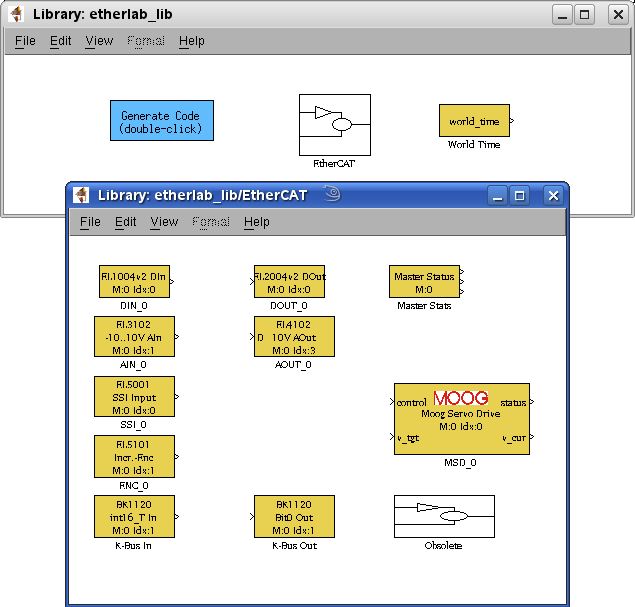
\includegraphics[width=0.9\textwidth]{images/blockset.png}
    \caption{EtherLab Simulink Blockset}
    \label{fig:blockset}
  \end{center}
\end{figure}

Figure~\ref{fig:el10xx} shows the configuration dialog for the
digital-input EtherCAT slaves of the Beckhoff EL10XX series.

\begin{figure}[H]
  \begin{center}
    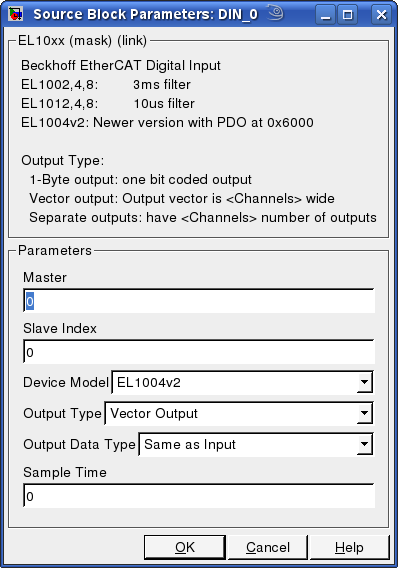
\includegraphics[width=0.4\textwidth]{images/el10xx.png}
    \caption{EL10xx configuration dialog}
    \label{fig:el10xx}
  \end{center}
\end{figure}

Figure~\ref{fig:el20xx} shows the configuration dialog for the
digital-output EtherCAT slaves of the Beckhoff EL20XX series.

\begin{figure}[H]
  \begin{center}
    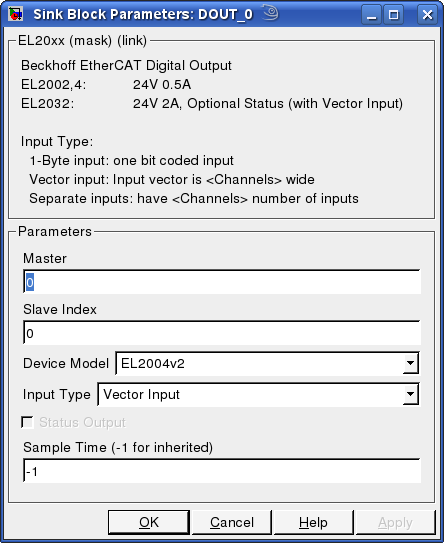
\includegraphics[width=0.4\textwidth]{images/el20xx.png}
    \caption{EL20xx configuration dialog}
    \label{fig:el20xx}
  \end{center}
\end{figure}

Figure~\ref{fig:el31xx} shows the configuration dialog for the
analog-input EtherCAT slaves of the Beckhoff EL31XX series.

\begin{figure}[H]
  \begin{center}
    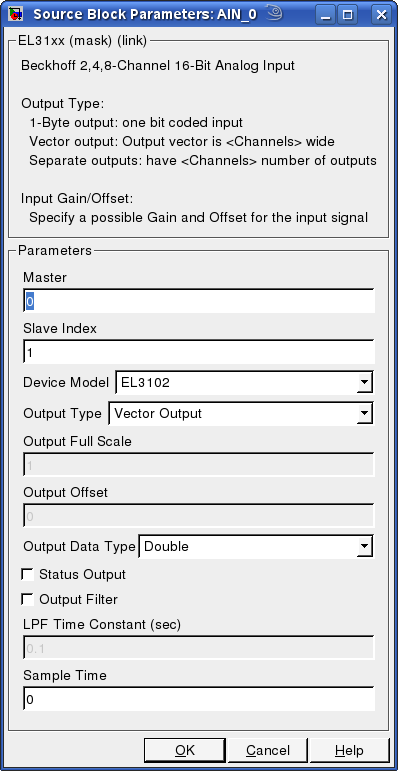
\includegraphics[width=0.4\textwidth]{images/el31xx.png}
    \caption{EL31xx configuration dialog}
    \label{fig:el31xx}
  \end{center}
\end{figure}

Figure~\ref{fig:el41xx} shows the configuration dialog for the
analog-output EtherCAT slaves of the Beckhoff EL41XX series.

\begin{figure}[H]
  \begin{center}
    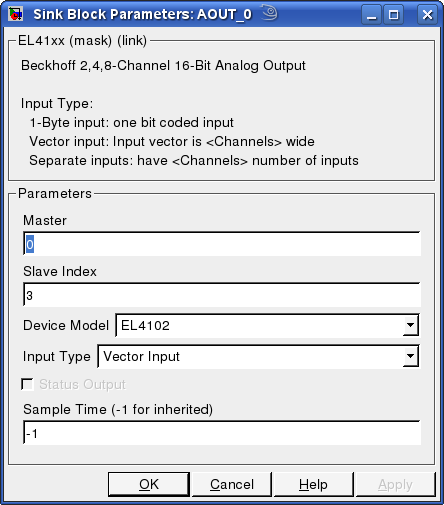
\includegraphics[width=0.4\textwidth]{images/el41xx.png}
    \caption{EL41xx configuration dialog}
    \label{fig:el41xx}
  \end{center}
\end{figure}

Figure~\ref{fig:el5001} shows the configuration dialog for the SSI
EtherCAT slave Beckhoff EL5001.

\begin{figure}[H]
  \begin{center}
    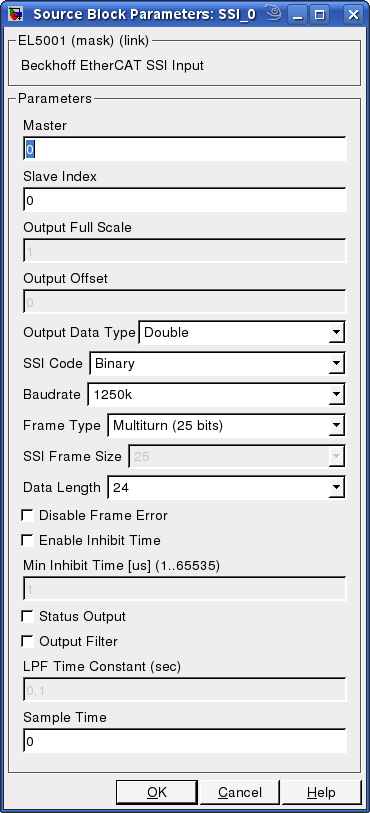
\includegraphics[width=0.4\textwidth]{images/el5001.png}
    \caption{EL5001 configuration dialog}
    \label{fig:el5001}
  \end{center}
\end{figure}

Figure~\ref{fig:el5101} shows the configuration dialog for the
incremental-encoder EtherCAT slave Beckhoff EL5101.

\begin{figure}[H]
  \begin{center}
    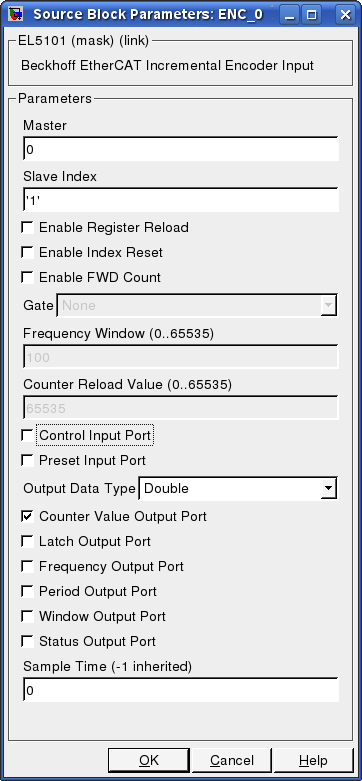
\includegraphics[width=0.4\textwidth]{images/el5101.png}
    \caption{EL5101 configuration dialog}
    \label{fig:el5101}
  \end{center}
\end{figure}

Figure~\ref{fig:bk1120-in} shows the configuration dialog for the Beckhoff
BK1120 EtherCAT-KBUS-coupler input block.

\begin{figure}[H]
  \begin{center}
    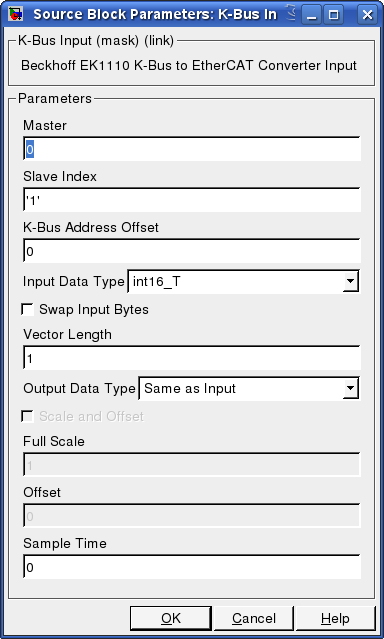
\includegraphics[width=0.4\textwidth]{images/bk1120-in.png}
    \caption{BK1120 input configuration}
    \label{fig:bk1120-in}
  \end{center}
\end{figure}

Figure~\ref{fig:bk1120-out} shows the configuration dialog for the Beckhoff
BK1120 EtherCAT-KBUS-coupler output block.

\begin{figure}[H]
  \begin{center}
    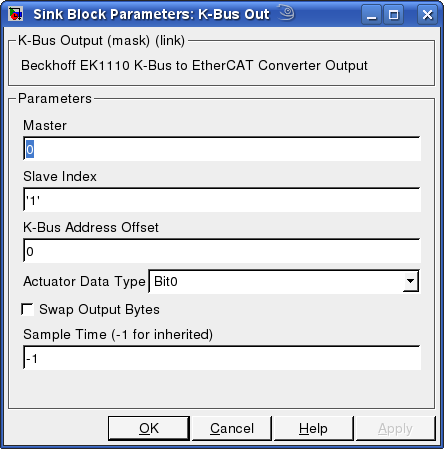
\includegraphics[width=0.4\textwidth]{images/bk1120-out.png}
    \caption{BK1120 output configuration}
    \label{fig:bk1120-out}
  \end{center}
\end{figure}

Figure~\ref{fig:msd} shows the configuration dialog for the MOOG servo drive
EtherCAT slave block. This block can be configured to be an input-only block,
an output-only block or and input/output block.

\begin{figure}[H]
  \begin{center}
    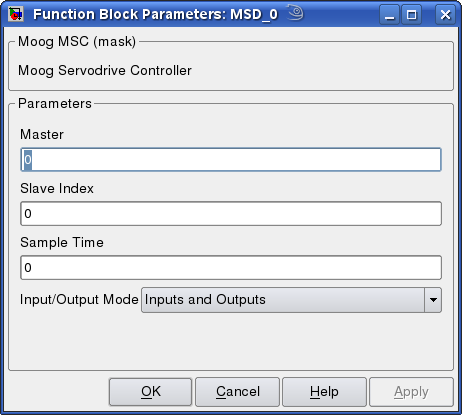
\includegraphics[width=0.4\textwidth]{images/moog_msd.png}
    \caption{MOOG servo drive configuration}
    \label{fig:msd}
  \end{center}
\end{figure}

Figure~\ref{fig:masterstats} shows the configuration dialog for the EtherCAT
master status block.

\begin{figure}[H]
  \begin{center}
    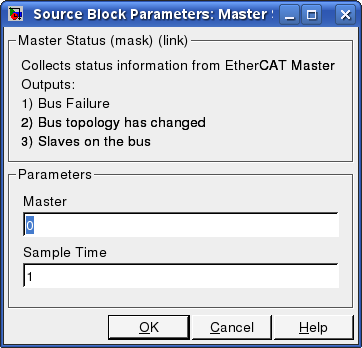
\includegraphics[width=0.4\textwidth]{images/master.png}
    \caption{Master status block configuration}
    \label{fig:masterstats}
  \end{center}
\end{figure}

\end{ighsec}

%-----------------------------------------------------------------------------

\begin{ighsec}{Creation of EtherLab Models with Simulink}
\label{sec:modelle}

After creating a new model sheet within Simulink, a few parameters have to be
set up (menu \textit{Simulation/Configuration Parameters\ldots}):

\begin{itemize}
\item The input field \textit{Realtime Workshop} $\rightarrow$
  \textit{System target file} must contain the file name
  \texttt{etherlab.tlc}. It can be chosen via the
  \textit{Browse\ldots} button (see figure~\ref{fig:konfiguration}).
  \begin{figure}[H]
    \begin{center}
      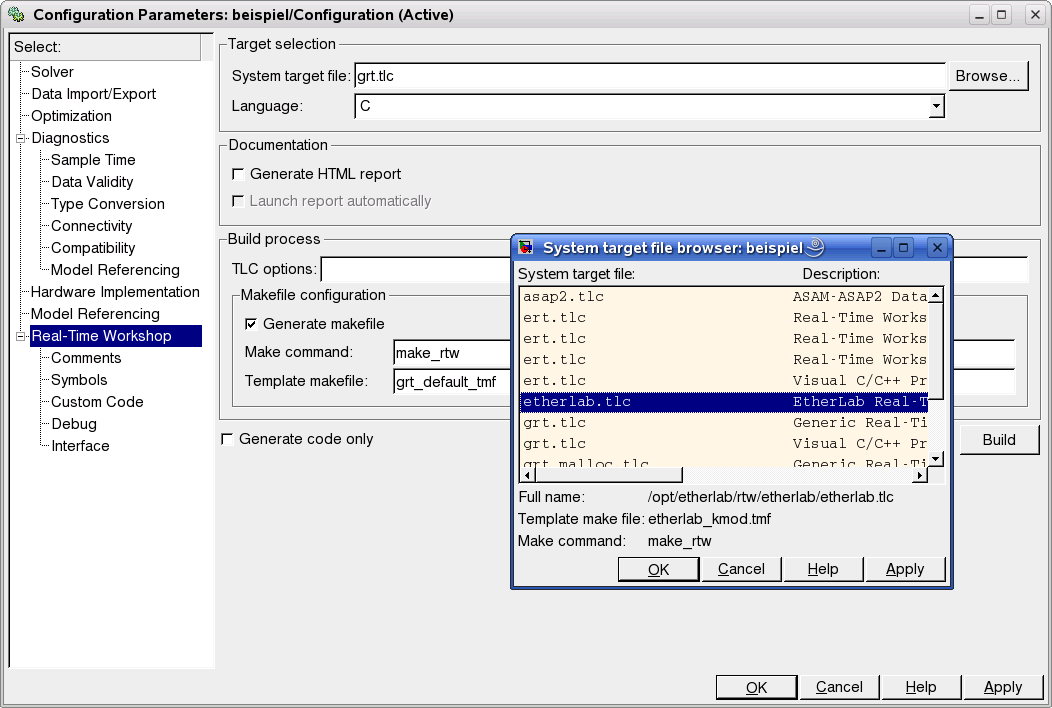
\includegraphics[width=.9\textwidth]{images/config_param.png}
      \caption{Configuration of model parameters}
      \label{fig:konfiguration}
    \end{center}
  \end{figure}
\item The input field \textit{Solver} $\rightarrow$ \textit{Fixed-step
    size} must contain the period time of the real time cycle, for
  example \texttt{0.01} meaning $100$ Hz (see
  figure~\ref{fig:config_solver}).
  \begin{figure}[H]
    \begin{center}
      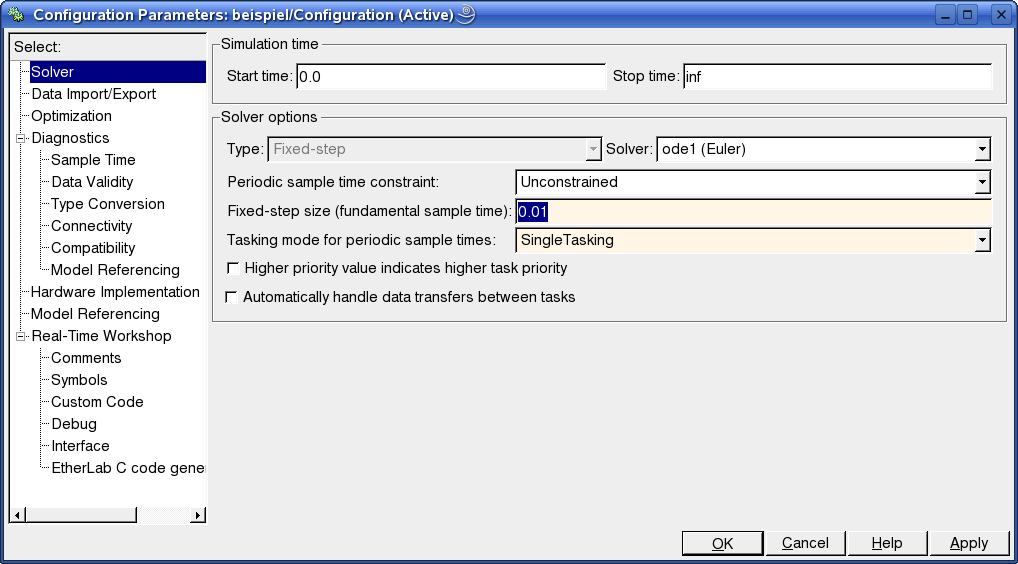
\includegraphics[width=.9\textwidth]{images/config_solver.png}
      \caption{Configuration of model parameters (2)}
      \label{fig:config_solver}
    \end{center}
  \end{figure}
\end{itemize}

After the model has been parametrized, it can be edited as usual. To use
EtherLab blocks, open the \texttt{etherlab\_lib} (see sec.~\ref{sec:lib})
and drag the desired blocks on the new model sheet. When finished,
\textit{Ctrl-B} will generate the model code including a Linux kernel module.

\end{ighsec}

%-----------------------------------------------------------------------------

\end{ighsec} % Simulink

%-----------------------------------------------------------------------------

\begin{ighsec}{Starting EtherLab Models}
\label{sec:start}

The \texttt{rt\_kernel} module must be inserted before inserting any EtherLab
modules. If EtherLab is configured as a service (see
section~\ref{sec:dienst}), this is done automatically at system startup.
Otherwise the module can be inserted manually. It is recommended to start the
module using the init script, because the necessary device files are then
created automatically:

\begin{lstlisting}
  # `\textbf{/opt/etherlab/etc/init.d/etherlab start}`
\end{lstlisting}

After that, an EtherLab module can be loaded.

\begin{lstlisting}
  # `\textbf{insmod <model>\_kmod.ko}`
\end{lstlisting}

If the \texttt{insmod} command returns with an error, the kernel ring
buffer can be analyzed for possible software or hardware
misconfigurations:

\begin{lstlisting}
  # `\textbf{dmesg | less}`
\end{lstlisting}

If the model was loaded successfully, its process variables (i.\,e.\,signals
and parameters) can ve accessed via TCP/IP with EtherLab tools like
Testmanager, DLS or the RTCom library (have a look at
\url{http://etherlab.org/en/components.php}. Therefore the
\texttt{etherlab\_buddy} acts as a TCP server listening on port 2345 and
communicating with an XML-based protocol called MSR (see the german
documentation at \url{http://etherlab.org/download/m-igh_rt_api.pdf}).

\end{ighsec}

%-----------------------------------------------------------------------------
